\section{Umsetzung}
\subsection{Softwarearchitektur}
     ein paar sätze zur Abbildung~\ref{fig:architecture}
     \begin{figure}[tbh]
            \centering
            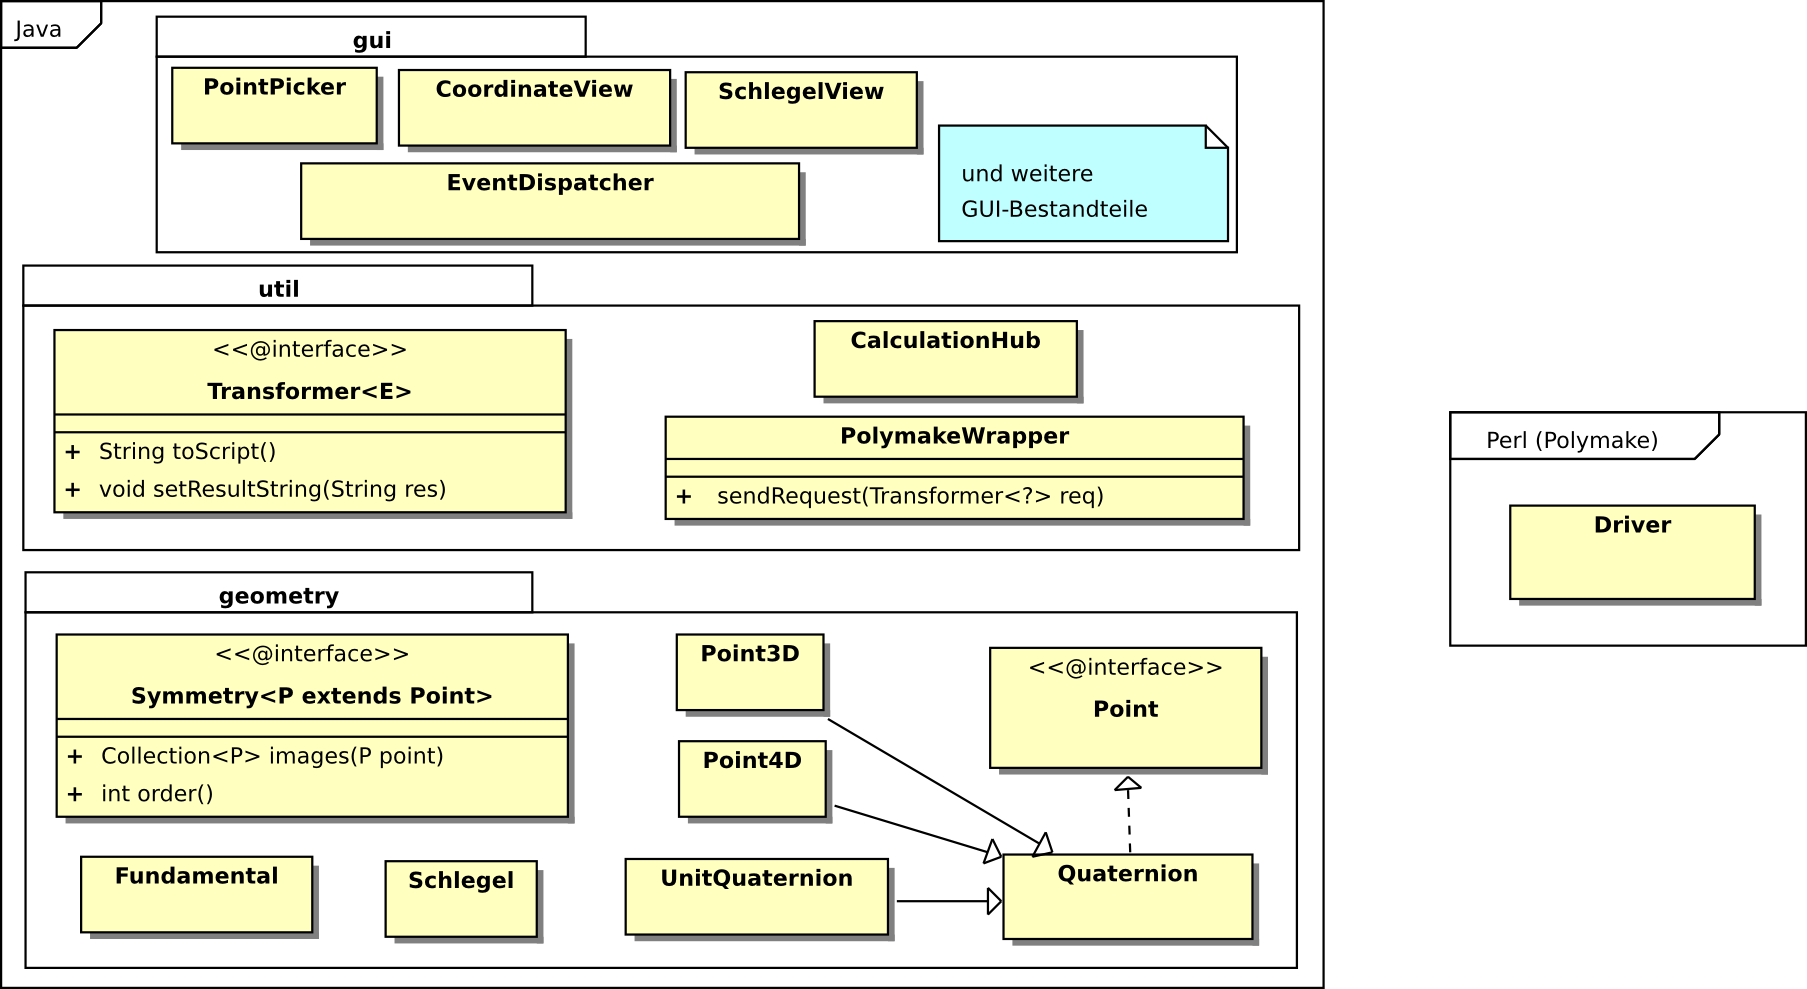
\includegraphics[width=0.85\textwidth]{img/architecture}
            \caption{Grobübersicht über die Architektur des Projekts\label{fig:architecture}}
        \end{figure}
    \begin{itemize}
        \item Pipeline-artiger Informationsfluss (siehe~\ref{ssec:flow})
        \item Lose Kopplung durch Eventsystem (siehe~\ref{ssec:event})
        \item Aufbereitung der Daten durch GUI (siehe~\ref{ssec:gui})
    \end{itemize}
    Grobidee skizzieren: Wir verwenden polymake als externen rechner und verwalten zustand/gui selbst. anzeige wird mit hilfe von jreality gemacht....integriert, blabla.

    \subsubsection{Verwendete Softwarehilfsmittel}
       \begin{itemize}
           \item jReality~\cite{jreality} jeweils 1-2 saetze was /wofür das ist
           \item polymake~\cite{polymake} jeweils 1-2 saetze was /wofür das ist
           \item maven~\cite{maven} jeweils 1-2 saetze was /wofür das ist
           \item jUnit jeweils 1-2 saetze was /wofür das ist
        \end{itemize}

    \subsubsection{Informationsfluss\label{ssec:flow}}
        \begin{figure}[tbh]
            \centering
            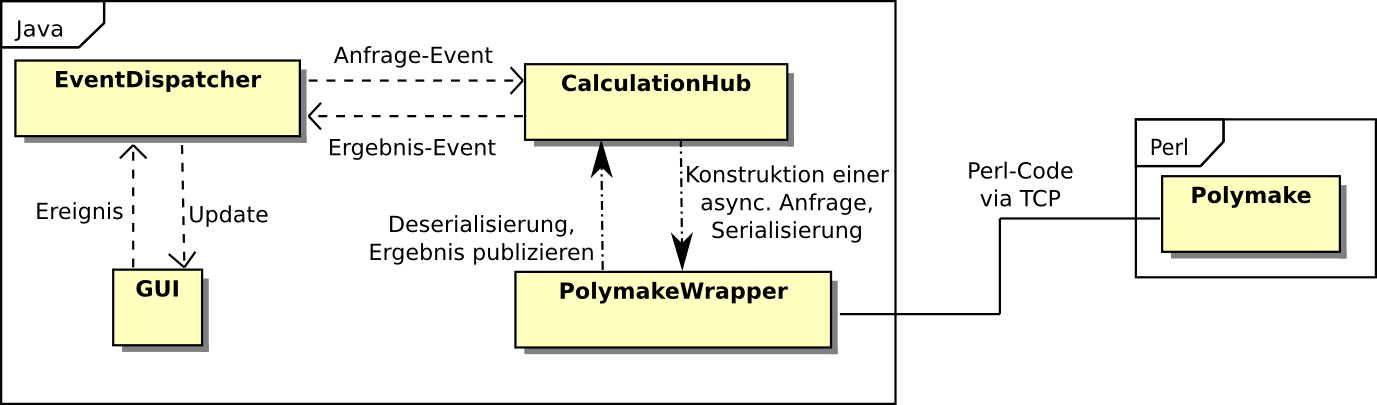
\includegraphics[width=0.85\textwidth]{img/flow}
            \caption{Informationsfluss zwischen den Komponenten
                      {\scriptsize(gestrichelt: sync. Methodenaufruf, punkt-strich: async. Methodenaufruf, durchgezogen: TCP-Nachricht}}
        \end{figure}

        yada yada 
    \subsubsection{Eventssystem\label{ssec:event}}
        \begin{figure}[bht]
            \centering
            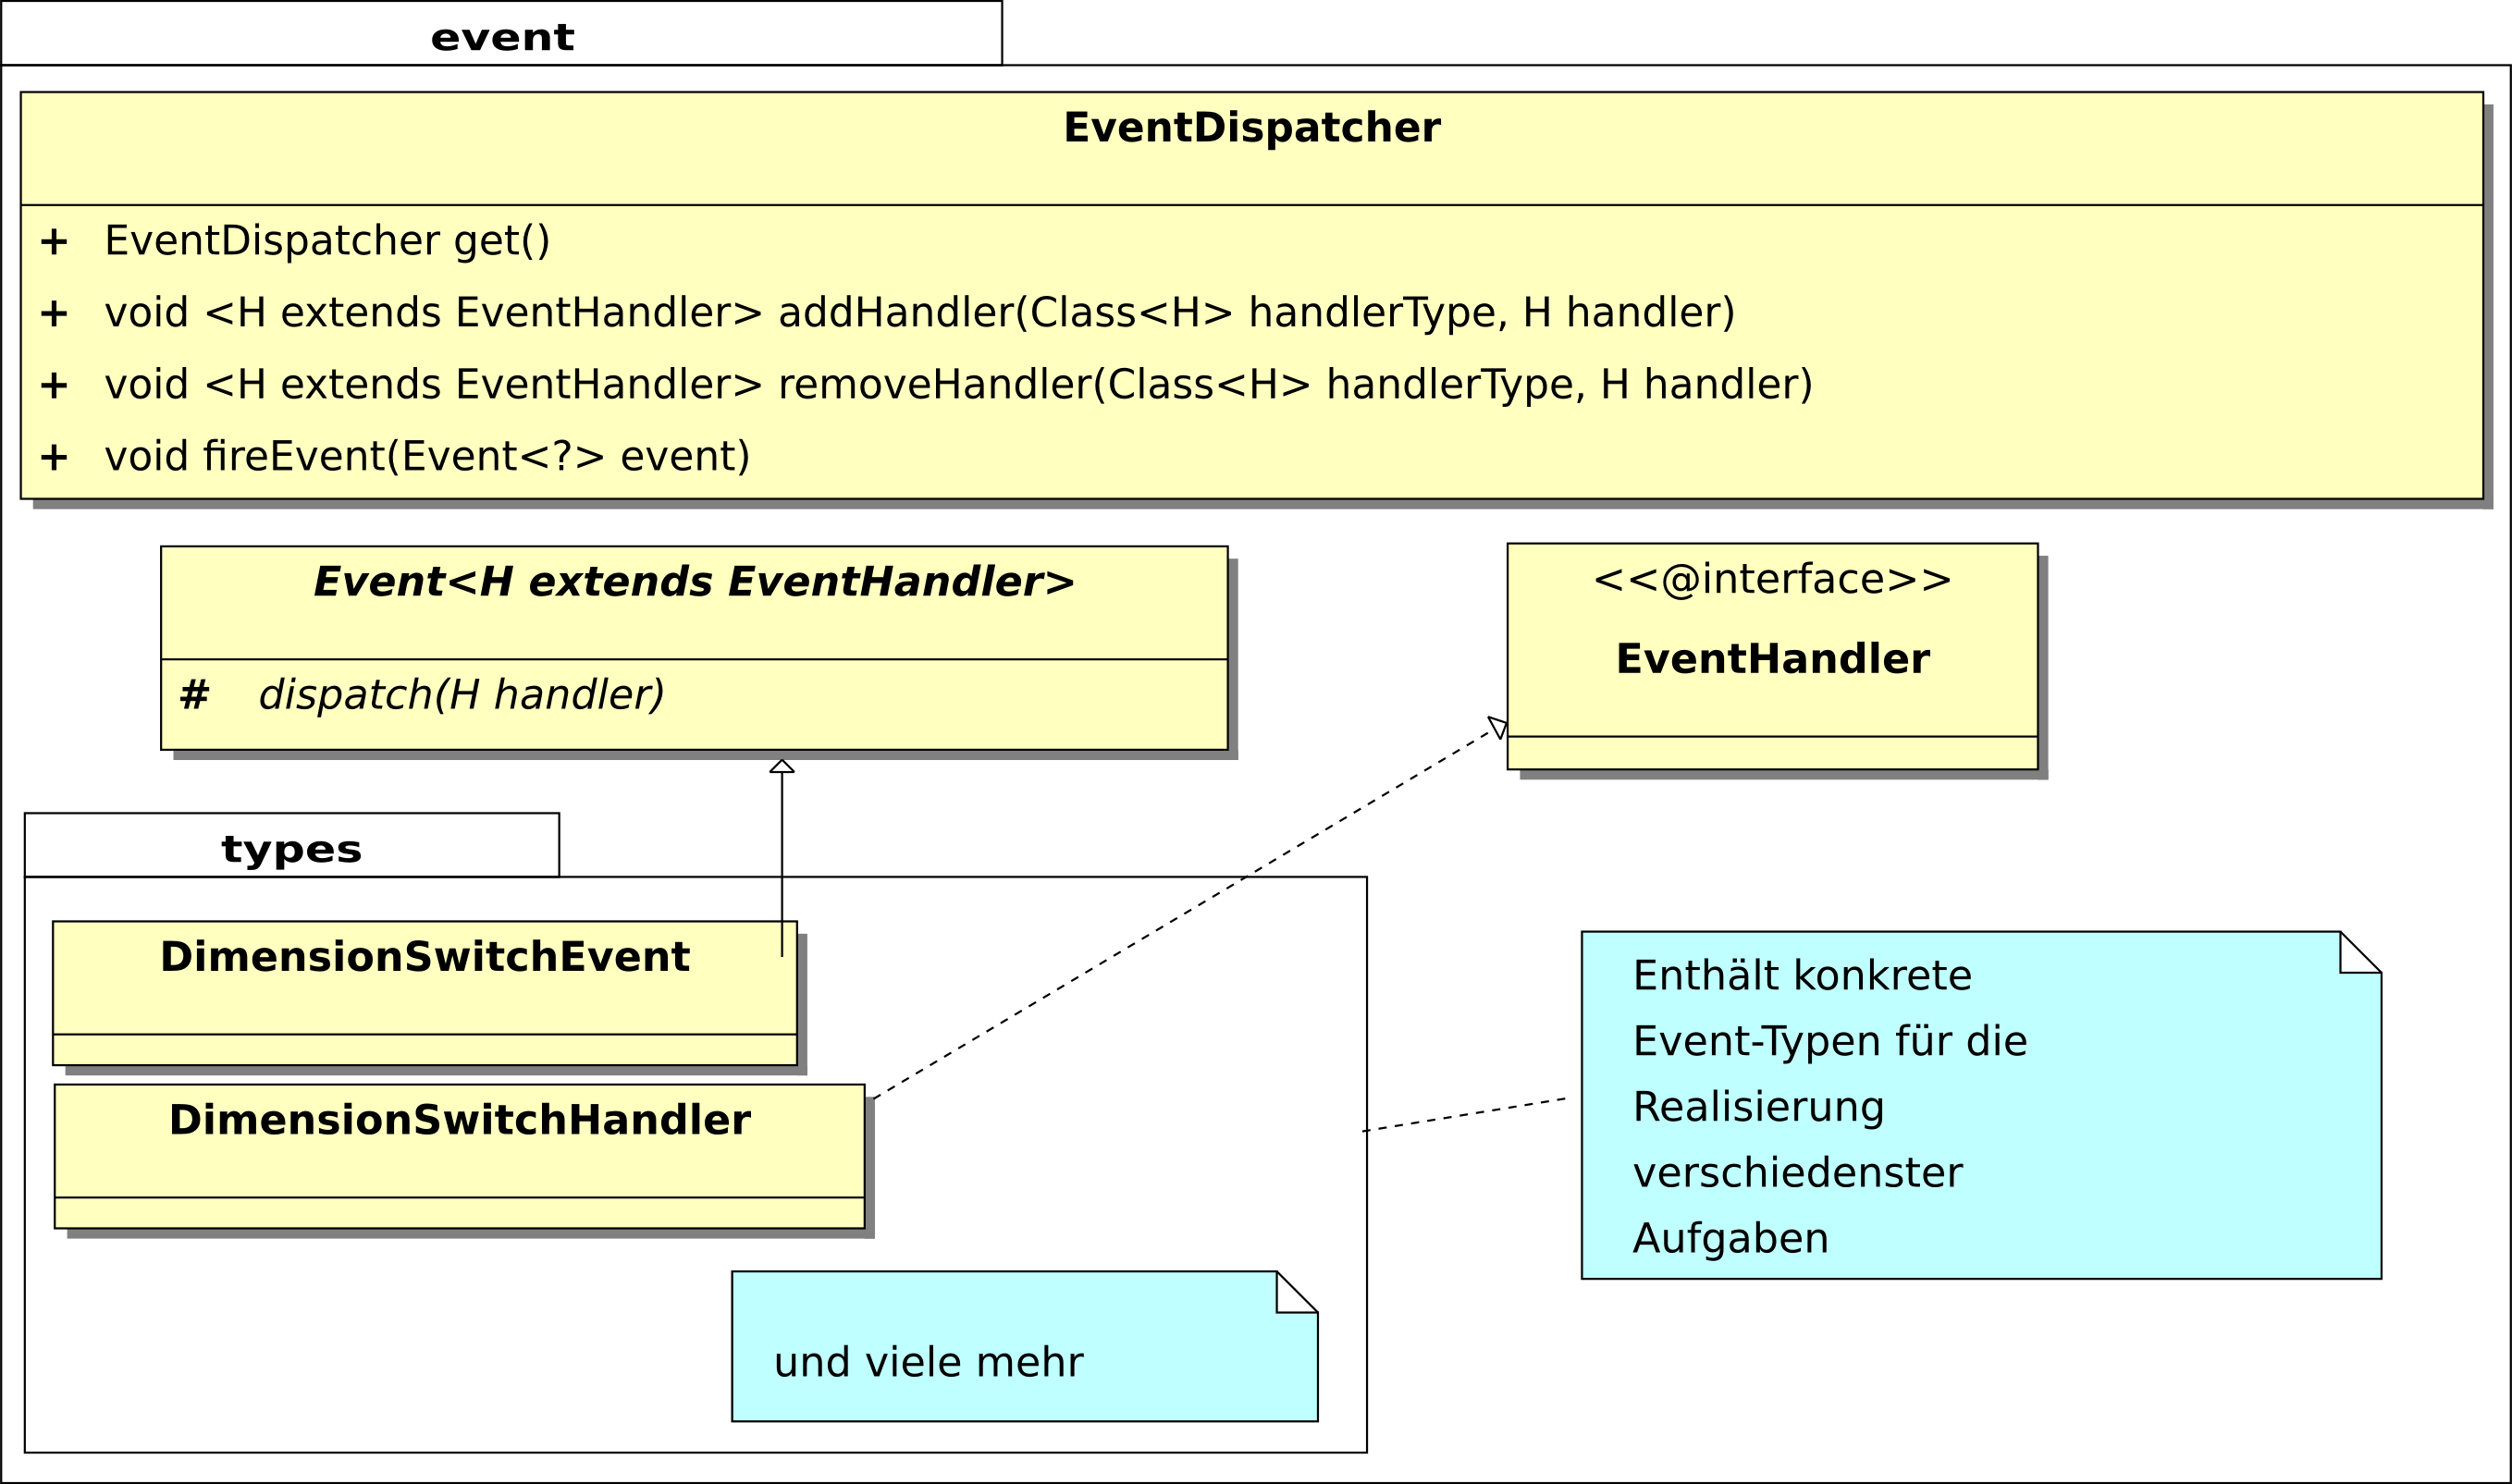
\includegraphics[width=0.8\textwidth]{img/event_classdiagram2}
            \caption{Klassendiagramm des Eventsystems}
        \end{figure}
        \subsubsection*{Events}
            Events sind konkrete Reaktionen auf bestimmte Ereignisse und enthalten je nach Ereignis entsprechende Kontextinformationen.
            Alle Typen von Events erben von der abstrakten Klasse \lstinline|Event<H extends EventHandler>| und stellen einen
            zugehörigen \lstinline|EventHandler|-Typen bereit.
            Komponenten, die auf ein bestimmtes Event reagieren sollen, realisieren das zum Event zugeordnete
            \lstinline|EventHandler|-Interface und implementieren damit eine Reaktionsmethode mit komponentenspezifischem
            Code.

            Eine zentrale Singleton-Instanz, der \lstinline|EventDispatcher|, koordiniert dann das Absenden und Empfangen von Events
            und verteilt die Ereignismeldungen an Interessenten.
            Hierfür muss jede an einem spezifischen Event interessierte Komponente sich als solche beim
            \lstinline|EventDispatcher| registrieren (\lstinline|addHandler(Class<H> eventType, H handler)|).
            Eine designierte Eventquelle hält ebenfalls einen Verweis, um mittels dessen
            \lstinline|fireEvent(Event<?> e)|-Methode im Zuge einer Reaktion ein Event abzufeuern.

      %  \subsubsection*{Eventimplementierung}
      %      Event-Typen werden durch Anlegen einer Event-Klasse und einer EventHandler-Klasse hinzugefügt.%
%
%            Das EventHandler-Template ist
%            
%            \begin{code}
%                import pointGroups.gui.event.EventHandler;
%
%                public interface ConcreteHandler
%                    extends EventHandler
%                {
%                    public void onConcreteEvent(final ConcreteEvent event);
%                }
%            \end{code}
%
%            Das Event-Typ-Template ist
%
%            \begin{code}            
%                import pointGroups.gui.event.Event;
%
%                public class ConcreteEvent
%                    extends Event<ConcreteHandler>
%                {
%                    public final static Class<ConcreteHandler> TYPE =
%                        ConcreteHandler.class;
%
%                    @Override
%                    public final Class<ConcreteHandler> getType() {
%                        return TYPE;
%                    }
%
%                    @Override
%                    protected void dispatch(final ConcreteHandler handler) {
%                        handler.onConcreteEvent(this);
%                    }
%                } 
%            \end{code}
%            
%            wobei Concrete durch konkrete Namen ersetzt werden kann.
            
        \subsubsection{GUI\label{ssec:gui}}
             MARCEL: ein bisschen erzählen, woher jreality kommt und warum wir es benutzen (in frame eingebettet etc). was es kann, wie wir es bisschen anpassen mussten.
                
\subsection{Implementierung von Berechnungen}
    \subsubsection{Symmetriebilder}
        ALEX SCHREIBT HIER KURZEN PSEUDOCODE    
    \subsubsection{Symmetriegruppen}
    Eine Symmetriegruppe wird durch einen Enum repräsentiert. Durch diesen Enum wird auf Hashmaps zugegriffen. Es gibt jeweils eine Hashmap für die Gruppenelemente und die Untergruppen. Dies erleichert das Hinzufügen von Symmetriegruppen, deren Zugriff und die Verwaltung von Gruppenelementen. Es ist im Gegensatz zu unserem ursprünglichen Entwurf nur eine Klasse für den dreidimensionalen Fall nötig und es erspart deutliche Redundanzen. Dies betrifft insbesondere die Nutzung von Gruppenelementen und die Untergruppenbeziehungen. Dieser Entwurf ist somit leichter wartbarer und wiederbenutzbarer.
    Für die Nutzung der Symmetriegruppen steht ein Interface bereit, welches einen leichten und intuitiven Zugang ermöglicht. Die wesentlichen Funktionen sind die Ausgabe der verschiedenen Bezeichnungen einer Gruppe, die Ordnung, die Untergruppen und die Berechnung der Punktgruppe zu einem gegebenen Punkt. Dies war besonders beim Entwurfswechsel sinnvoll. Denn so musste im restlichen Quellcode beim Entwurfswechsel nur sehr wenige Änderungen vorgenommen werden. Dieses Interface wird sowohl für den dreidimensionalen Fall sowie für den vierdimensionalen Fall verwendet.\\ 
    %%3D case
    Die dreidimensionalen Symmetriegruppen sind ausgiebig dokumentiert und nicht sehr umfangreich im Vergleich zum vierdimensionalen Fall. Wir konnten dort die Gruppenelemente als auch die Untergruppen fest einprogrammieren. \todo{Beispielcode} \\
        OLLI SCHREIBT HIER ZU .... Symmetriegruppen (Berechnung mittels Generatoren, hart kodiert, Darstellung/Repräsentation)
%%%% 4D-case
Im vierdimensionalen Fall waren die Symmetriegruppen nur durch die Generatoren beschrieben und eine händische oder halbautomatische Erzeugung erscheint bei den Gruppengröße von teilweise einigen tausend Elementen nicht sinnvoll. Wir haben uns dazu für die Erzeugung mittels Gruppen entschieden. Dies ist nachträglich für den dreidimensionalen Fall auch möglich und die Ergebnisse wurden in diesem Fall auch verifiziert.\\
Die Grundlage für unseren Algorithmus ist das Hintereinanderausführen der Erzeuger und die Speicherung von neuen Elementen. Das Hauptproblem dabei ist das Überprüfen, ob ein Element bereits in einer Gruppe vorhanden ist. Bei Gruppen von mehreren tausend Elementen ist eine naive Suche zu zeitintensiv und es kann zu Rundungsfehlern kommen. Aus diesem Grund haben wir uns für eine Hashmap zur Speicherung der Elemente entschieden. Dazu mussten für eine Rotation eine Hashmethode erzeugt werden. Die Anforderungen an die Hashmethode musste eine schnelle Berechnung ermöglichen, im Einklang mit einer equal-Methode sein und eine gute Streuung der Elemente garantieren.\todo{Formulierung?}
\subsection{Symmetriegruppen im 4D}
\begin{itemize}
	\item Berechnung mittels Generatoren
	\item Rotation4D klasse
	\item hashcode und equals methoden
	\item Gitternetz
	\item Testfälle mittels Gruppengröße
	\item Speicherung
	\item Untergruppenbeziehungen
	\item Testfälle Untergruppenbeziehungen
	\item Berechnung
\end{itemize}


    \subsubsection{Fundamentalbereich}
         In Abschnitt \ref{fundamentalbereich} wurde in Definition \ref{fundamentalbereich:voronoi} der Voronoi-Fundamentalbereich beschrieben. Wir wollen eine dieser Zellen
         nehmen und Visualisieren. Da wir einen Abschnitt der $S^3$ nicht leicht visualsieren können, benötigen wir zunächst eine Projektion das Vornoi-Fundamentalbereiches auf
         eine $\mathbb{R}^3$ Ebene.
        \subsubsection*{Idee}
            Wir lassen zunächst die Gruppe auf ein Ausgezeichnetes Element $x$ wirken.

            Als erstes Berechnen wir die Voronoi - Zelle für $x$ bezüglich des Orbits von $x$. Alle Punkte die dort drinnen liegen sind Elemente von $S^3$. Da die Gruppe symmet          risch ist, können wir nicht zwei Elemente aus dem selben Orbit haben, da der zweite Punkt näher an einem anderen Element aus $G \rhd x$ liegen müsste.

         Das einzig wichtige an diesem Punkt ist, dass $x$ nicht auf einer Rotationasachse oder Spiegelebene befindet, da sonst die Voronoizellen zu groß ausfallen.

         Haben wir diese Zelle, nehmen wir eine beliebige Ebene, die tangential auf dem Kugelsegment ist und projezieren darauf. Die spezielle Ebene, die wir wählen
         ist die Ebene $h \, : \, [t - x] \cdot x = 0$ in Normalendarstellung, da wir wissen, dass $x$ auf der Kugeloberfläche im Kreissegment liegt und $x$ auch ein
          Normalenvektor ist.
            
        \subsubsection*{Umsetzung}
         Eine Voronoizelle von $x$ für eine Menge von Sites $S$ ist definiert als 
         $$ VC(x) = \bigcap_{s \in S \setminus \{ x \}} h^+_{x,s}$$
         Wobei $h^+_{x,s}$ der Halbraum ist, der rechts von der Hyperebene liegt, die zu $x$ und $y$ in jedem Punkt den selben Abstand hat.\\

         Polymake hat die Möglichkeit ein Polytope, das die Voronoizelle ja ist, gerade über den Schnitt von Halbräumen zu definieren. Dies geht über

         \begin{code}
            new Polytope(INEQUALITIES=>\$hyperplanes)
         \end{code}

         wobei \$hyperplanes eine Menge von Hyperebenen ist. Falls ein affines Polytope vorliegt, wie in unserem Fall in der Ebene $h$, die wie im letzten Abschnitt
         definiert ist, können wir auch dies mit in die Erzeugung eingeben mittels

         \begin{code}
            new Polytope(INEQUALITIES=>\$hyperplanes, EQUATIONS=>{h})
         \end{code}

         und haben so $VC(x)$ berechnet. Da die konkrete Berechnung über den Schnitt von allen Hyperebenen zu lange dauert, filtern wir die in frage kommenden Hyperebenen vor
         über die Nachbern des Voronoi Diagrams. Dummerweise konnten wir nicht ermitteln, wie man in Polymake sich direkt eine Voronoizelle ausgeben lassen kann und
         haben daher diesen Umweg gewählt.\\

         Haben wir nun das Polytope in der Ebene, müssen wir zur Darstellung in $n-1$ Dimensionen noch eine geeignete Basis berechnen, so dass wir
         die Eckpunkte des Polytopes durch $n-1$ Koordinaten darstellen können. Wir wissen schon, dass $x$ senkrecht auf der Ebene steht, also für unsere Darstellung 
         unerheblich ist. Wir berechnen eine Orthonormalbasis für die Ebene mit $x$ als erstem Basisvektor. Nun können wir leicht eine Basiswechselmatrix angeben,
         da wir ja die Bilder der neuen Basis in der alten kennen. Darüber hinaus ist diese Matrix orthogonal -- da die Spalten ja eine orthogonal Basis waren -- und
         kann daher durch transponieren invertiert werden.

         Wir haben nun also zwei Matrizen um beide Darstellungen in einander umzurechnen. In der neuen Basis können wir nun die erste Komponente weg lassen,
         da diese nach Projektion nur genullt wird und haben so eine Darstellung in $n-1$ Dimensionen.

         Beim zurückrechnen müssen wir uns nur erinnern, dass wir uns in einer affinen Ebene mit Stützvektor $x$ befinden.

        \subsubsection*{Berechnung}

         Die Hyperebenen Definition in Polymake hat die Darstellung
         $$
            h \, : \, [a_0, ..., a_n] \rightsquigarrow a_0 + a_1 x_1 + \cdots + a_n x_n = 0
         $$
         und Halbräume ebenso mit $\geq 0$.\\

         Die Halbräume für unser Polytope genügen der Gleichung
         $$
            t \cdot (x - s) \geq 0 \Leftrightarrow 0 + (x_1-s_1)\cdot t_1 + \cdots + (x_n -s_n)t_n \geq 0
         $$
         wobei $x$ der gewählte Vektor war und $s \not x$ aus dem Orbit von $x$ stammt.

         Damit können wir alle Halbräume aus dem Orbit berechnen. Die affine Ebene genügt der Gleichung
         $$
            (t - x) \cdot x = 0 \Leftrightarrow - \left( \sum_{i=1}^n x_i^2 \right) + t_1 x_1 + \cdots t_n x_n = 0
         $$
         und kann auch leicht erstellt werden. Um an unser Polytope heran zu kommen, benutzen wir das folgende Polymake-Script

         \begin{code}
            my \$poly = new Polytope(INEQUALITIES=>\$hyperplanes, EQUATIONS=>\$affine);
            print \$poly->VERTICES;
            print \$poly->EDGES;
            print \$poly->FACETS;
         \end{code}

         Mit diesen Ergebnissen können wir nun die Basiswechselmatrizen berechnen und so die Vertices umrechnen. Das Object Fundamental ist somit
         eine Sammlung dieser Eigenschaften.

         \begin{code}
            public interface Fundamental {
               public double[][] getVertices();
               
               public Edge<Integer,Integer>[] getEdges();

               public double[] revertPoint(double[] point);

               public boolean inFundamental(double[] point);
            }
         \end{code}
         
         Die ersten beiden Funktionen sind selbst erklärend. Die dritte methode \emph{revertPoint} nimmt einen Punkt in $\mathbb{R}^{n-1}$ und
         liftet ihn auf die Oberfläche der $S^{n-1}$ zurück. Die letzte Methode überprüft, ob ein angegebener Punkt überhaupt in der Voronoizelle lag.
         Diese Methode wird bei der anzeige beötigt um bei der Punktauswahl keine Punkte außerhalb das Polytops zuzulassen.\\

         Das ganze ist ein interface, da wir als Fallback-case, falls die Berechnung das Fundamentalbereichs einmal fehl schlägt immer noch 
         den Bereich $S^{n-2}$ benutzen können. Dies ist kein Fundamentalbereich, da wir alle Orbite mehrfach treffen, allerdings werden wir außer im Falle
         der Identität wirklich jeden Orbit mindestens einmal treffen.
